
\subsection{Implementation}

%% track selection

In addition to the track selection described in Section~\ref{sec:samples}, tracks fed to the RNN are required to pass additional quality requirements identical to those required by IP3D: track $p_{T} > 1$ GeV, $| d_0 | <1$ mm and $| z_0 \sin \theta | <1.5$ mm, and seven or more silicon hits, with at most two silicon holes, at most one of which is in the pixel detector,
where a hole is defined as a hit expected to be associated with the track but not present.

For each selected track, the variables provided to the network can be found in Table~\ref{tab:rnn_vars}, and the architecture is represented schematically in Figure~\ref{fig:rnn}.
Initial tests showed that a network using only $\sdip$, $\szip$, and the track category outperformed IP3D, indicating that the RNN algorithm alone adds discrimination over a likelihood-based algorithm.
Adding the fraction of jet energy carried by each track, $\ptfrac$, and the angular separation between the track and jet axis, $\drtj$ improve this performance further.
One of the input variables, the track category, is an integer used by the IP3D algorithm to define categories of tracks with similar reconstruction quality and resolution.  As the numerical values of the categories have no relative meaning, the category is embedded into a trainable, unit-normalized, 2D continuous representation.
%is embedded into a unit normalized 2D continuous vector whose direction (for each category) was optimized as part of the network training.

\begin{table}[htbp]
\small
\begin{center}
  \tabulinesep=1.5mm
  \begin{tabu}{X[-1,l,m] | X[L,m]}
\hline
   Track Variable  &  Description \\ \hline
   \hline
   \multicolumn{2}{c}{Used in IP3D and RNN tager} \\ \hline
$\sdip$	& Lifetime signed transverse impact parameter significance, $d_{0} / \sigma_{d_0}$,
			 where $d_0$ is the transverse displacement at the point of closest approach to the
			 primary vertex, $ \sigma_{d_0}$ is the error on $d_0$, and the sign is defined to be
			 positive (negative)  if the point of closest approach to the primary vertex
			 is in front (behind) the primary vertex with respect to the jet direction. \\ \hline 
$\szip$		& Lifetime signed longitudinal impact parameter significance, $z_{0} / \sigma_{z_0}$, 
			 where $z_0$ is the longitudinal displacement at the point of closest approach to the
			 primary vertex, $ \sigma_{z_0}$ is the error on $z_0$, and the sign is defined to be
			 positive (negative)  if the point of closest approach of the track to the primary vertex
			 is in front (behind) the primary vertex with respect to the jet direction. \\ \hline
Category \cite{ATL-PHYS-PUB-2015-022}		& A categorization of the tracks depending on the number of observed, expected,
			 or missing hits in the different layers of the silicon pixel and strip detectors.
			 The category organizes tracks into categories of different impact parameter resolutions.\\ \hline
       \hline
       \multicolumn{2}{c}{New to the RNN tagger} \\ \hline
$\ptfrac$	& The fraction of transverse momentum carried by the track relative to the jet, $p_{T}^{\rm track} / p_{T}^{\rm jet}$. \\
\hline
$\drtj$	& The angular distance between the track and the jet axis, 
						 $\sqrt{ (\phi_{\rm track} - \phi_{\rm jet})^2 +(\eta_{\rm track} - \eta_{\rm jet})^2} $.\\
\hline
\end{tabu}
\caption{Descriptions of track variables used in IP3D and the RNN tagger.}
\label{tab:rnn_vars}
\end{center}
\end{table}

After the initial selection and category embedding, tracks are ordered by $|\sdip|$ and passed to a LSTM cell which transforms the arbitrary-length track sequence to a 50 dimensional vector. This vector is then fed into a feed-forward fully-connected layer with four outputs corresponding to the $b$-jet, $c$-jet, light-jet, and $\tau$-jet probabilities ($p_b$, $p_c$, $p_{\textrm{light}}$, and $p_\tau$). To ensure that these outputs sum to 1 these four outputs are then fed through a final softmax layer.


%% The RNN $b$-tagging algorithms contains a single layer of LSTM with 50 units followed by a softmax layer for classification with four outputs ($p_b$, $p_c$, $p_{\textrm{light}}$, and $p_\tau$).

%% In the context of $b$-tagging, RNNs can be used to process sets of tracks associated to a jet.  When processing a step of variables in a sequence, RNNs build probability estimates conditioned on previous step, thereby encapsulating the structure and correlations of the sequence into the RNN output. Specifically, we use Long-Short-Term-Memory (LSTM) units in recurrent layers of neurons to process features of each track in the jet and use the output of the RNN after all tracks have been processed for classification.
\begin{figure}[htbp]
  \centering
  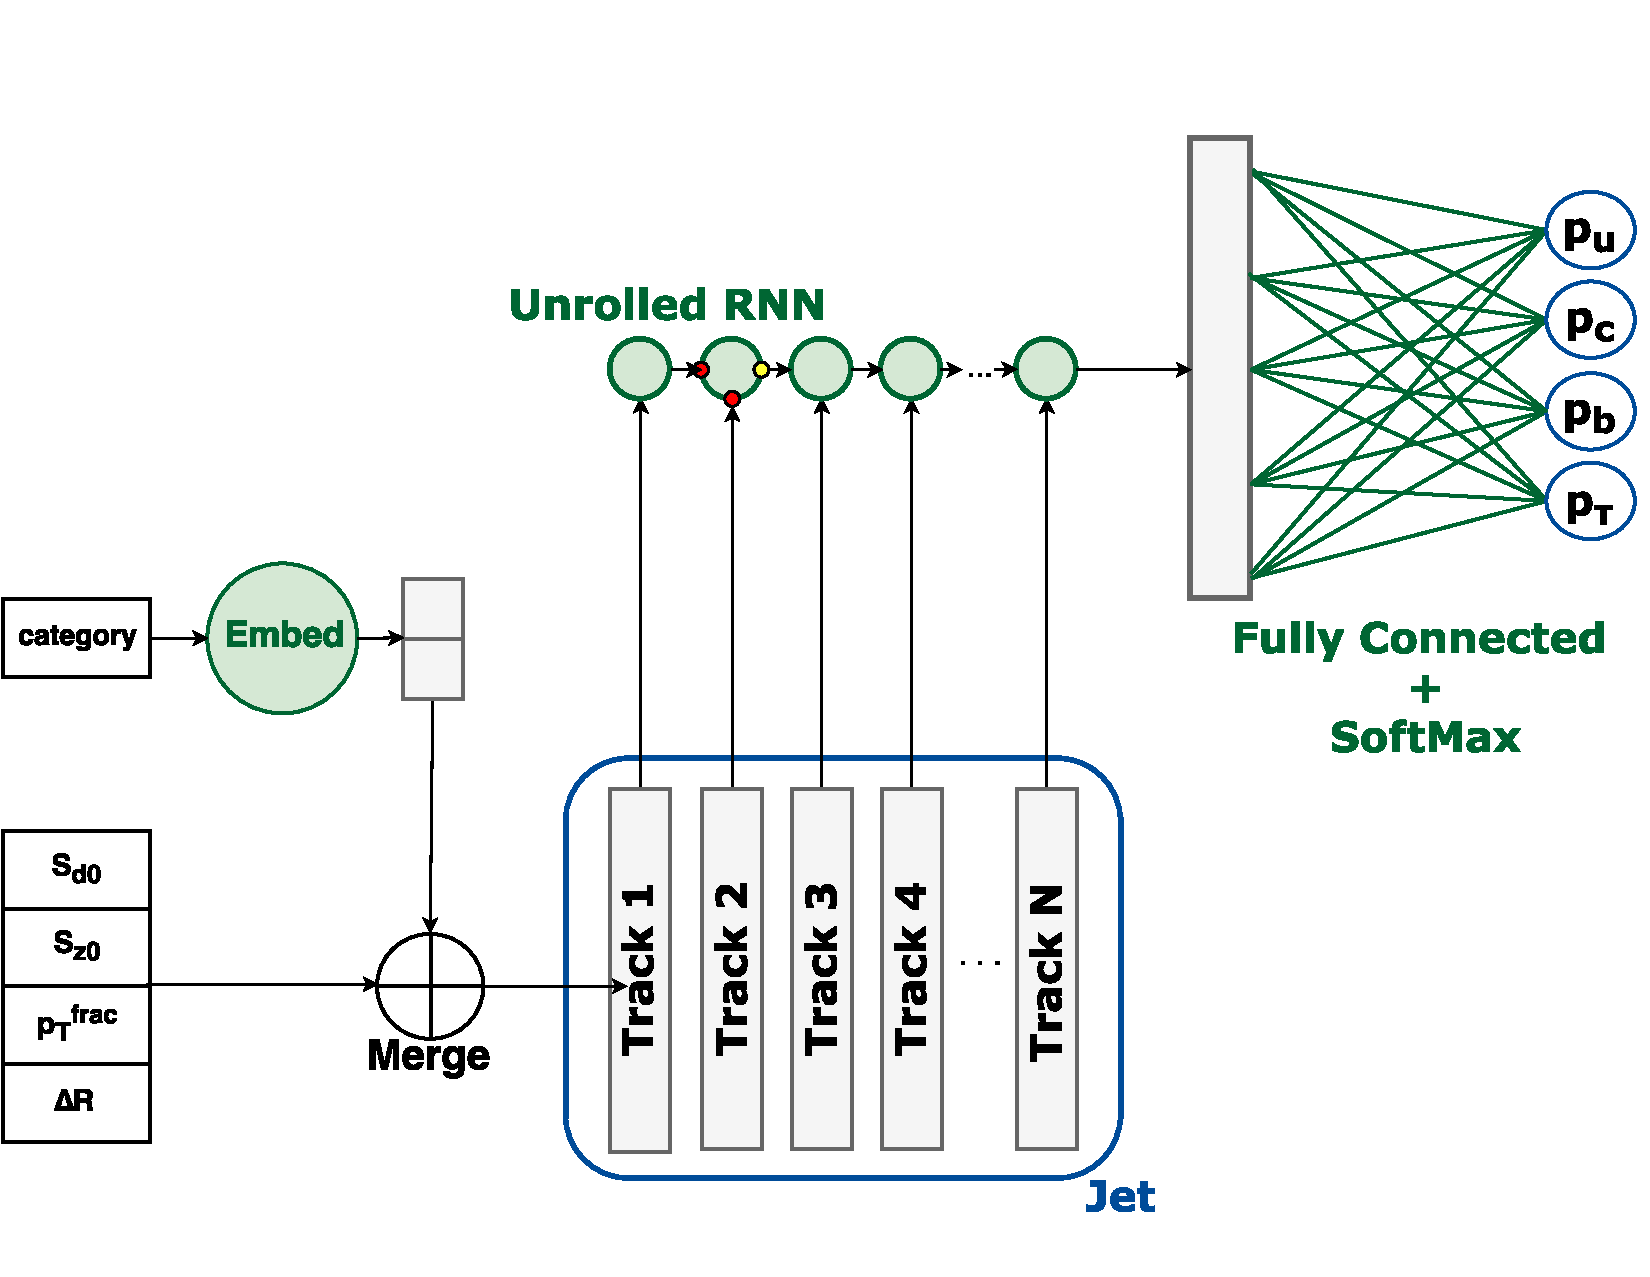
\includegraphics[width=\textwidth]{figures/RNN/RNNIP.pdf}
\caption{A schematic diagram of the RNN-based flavor-tagger.}
  \label{fig:rnn}
\end{figure}



%% Tracks are ordered by $|S_{d_{0}}|$.
The network was trained with 3.2 million jets, 7\% of which were $c$-jets\footnote{Changing this fraction has very little effect on the discriminant.}, and tested with an independent sample of 4 million jets. When evaluating the RNN, all tracks satisfying the quality criteria listed above are used, although for the sake of training the sequence was truncated at 15 tracks.
%~\todo{I would mention that this is okay because we expect the trailing tracks to be from background processes, so not much info is lost. Should we mention 0-padding at training time? or is it a technical detail?}
%% DAN: Zero padding is definitely just a detail.
Training with longer sequences showed negligible differences, which is unsurprising given that the chosen track ordering puts tracks from $b$-hadrons early in the sequence. The entire network was trained for 50 epochs using \textsc{Keras}~\cite{keras} with the \textsc{Theano}~\cite{theano} backend and the Adam optimizer~\cite{ref:ADAM}. Within the ATLAS event reconstruction software, the network is evaluated using \textsc{lwtnn}~\cite{lwtnn}.
%% on a CPU, and training time took $\sim 5$ hours.
When training, the jet transverse momentum spectrum of $b$-jets and separately $c$-jets were reweighted to the light-jet spectrum so as to prevent the neural network from learning to discriminate directly from sample and flavor specific momentum distributions.


In addition to the network described above, several related architectures were considered.
%% In order to treat the intrinsically unordered set of tracks as a sequence, other physics-inspired ordering schemes were investigated.
Ordering tracks by $|\sdip^2 + \szip^2|$ or $\pt$ showed minor differences in performance but no substantial benefit.
%% \todo{say something about nHits variant, maybe add to the table above. Also mention that bidirectional RNN showed promising improvement maybe?}
In another configuration, the 2D embedded track category was removed and replaced with the tracking variables which define track categories.
While this variant yielded similar performance,
the category embedding architecture was chosen because
the modeling of the IP3D categorization scheme in simulation has been more carefully scrutinized.
%% it could benefit from years of extensive studies indicating that the IP3D categorization scheme is accurately modeled in simulation.
Many other versions of the RNN presented above were examined, including different sets of track variables, alternative recurrent units, additional recurrent layers, additional fully-connected layers, and variations in the training parameters such as training epochs and learning rates.
The above network was ultimately found to perform better than or as well as others when accounting for classification accuracy, training time, and simplicity.

